
\documentclass[10pt]{article}
\usepackage[utf8]{inputenc}
\usepackage{graphicx}
\usepackage{amsmath, amssymb}
\usepackage{geometry}
\usepackage{caption} 
\geometry{a4paper, margin=0.5in, landscape} 

\begin{document}

\section*{Comparative EIS Kinetics Report}
\textbf{Model Structure:} \texttt{R0-p(R1-p(R2,CPE2),CPE1)} \\
\textbf{Used data:} altered data, first 2 points removed and points with $freq > 2e+04$ removed

\begin{center}
    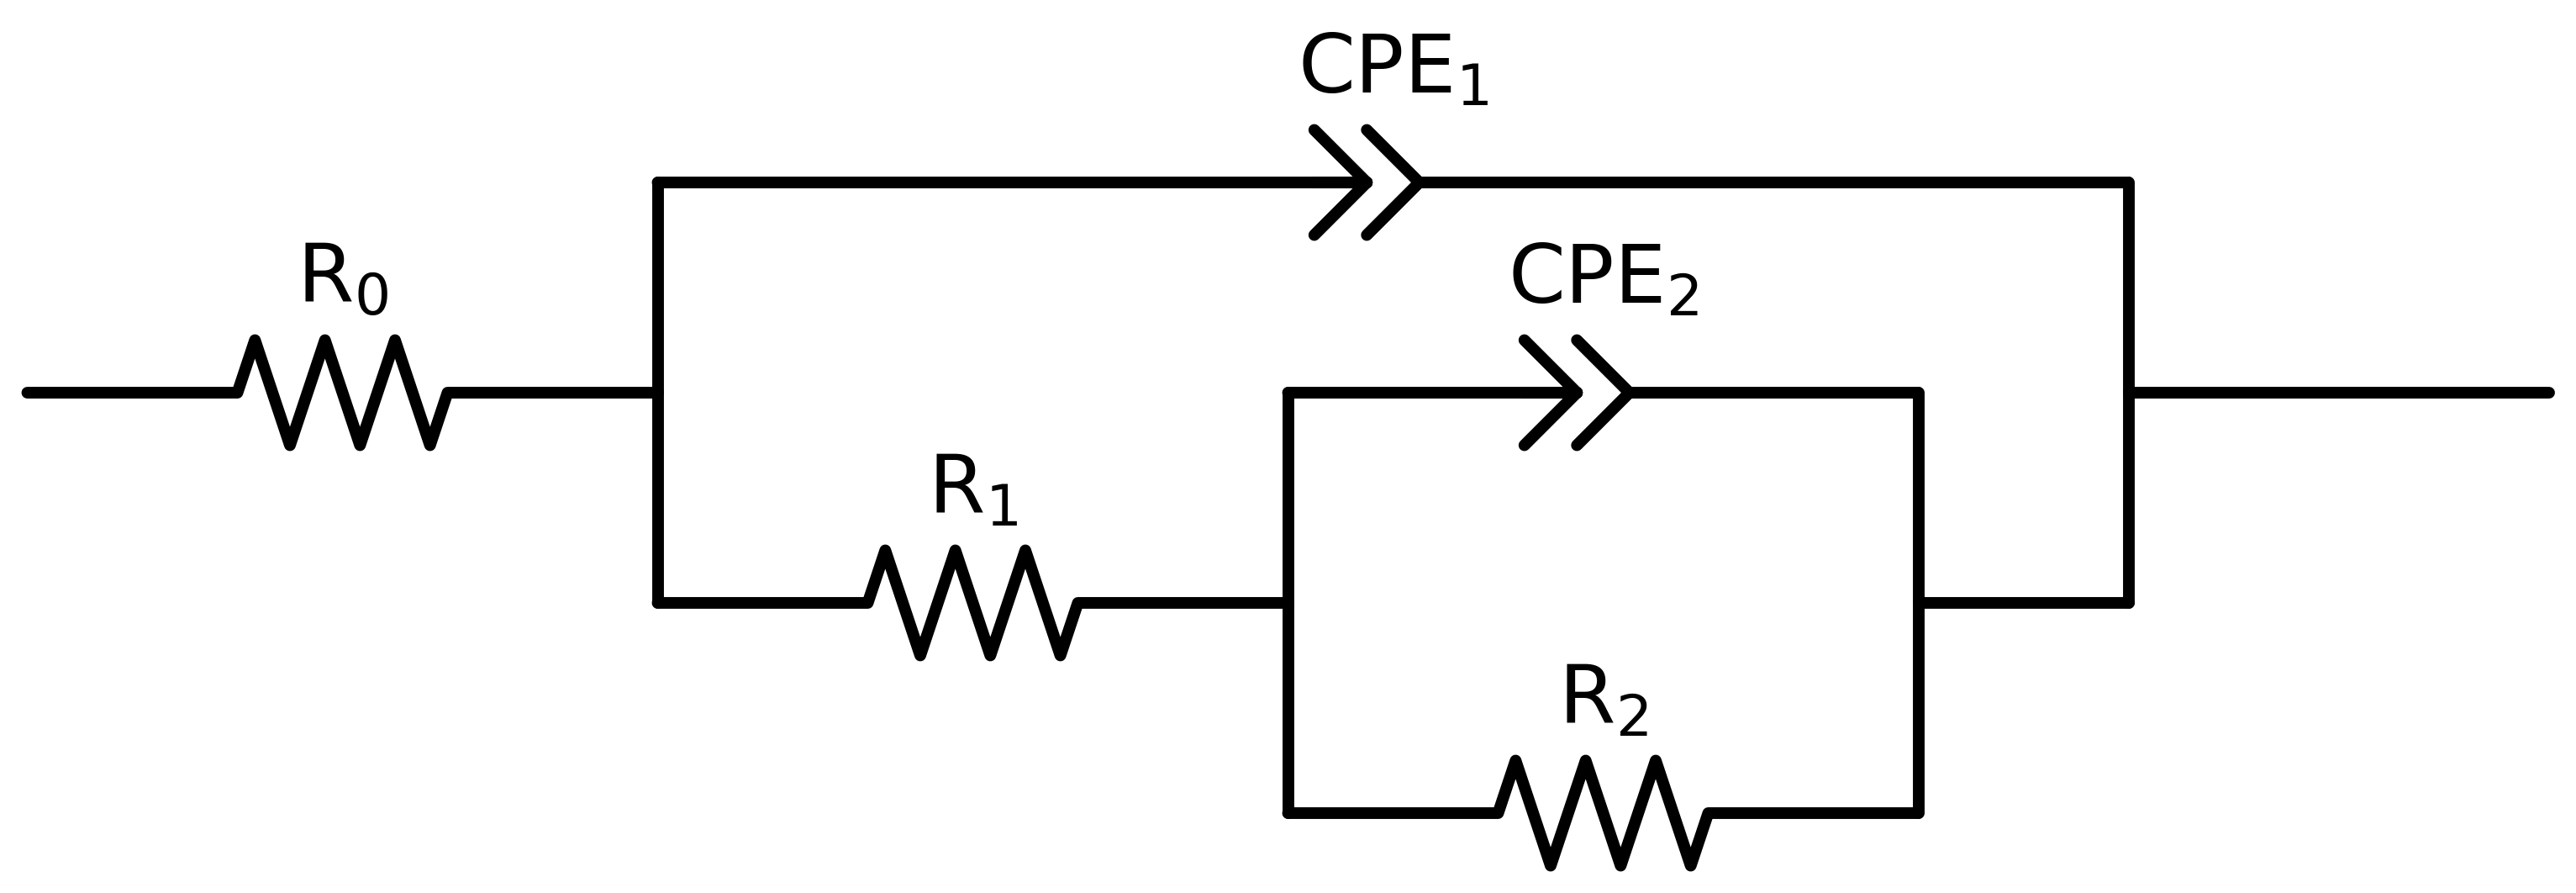
\includegraphics[width=0.45\textwidth]{../../2RC.png}
\end{center}

\renewcommand{\arraystretch}{1.6} 
\begin{table}[h!]
    \centering
    \footnotesize
    \begin{tabular}{|l|c|c|c|c|c|c|}
        \hline
        \textbf{Element} & \textbf{Unit} & \textbf{Bounds} & \textbf{Cauvel\_1\_MBT\_24H} & \textbf{Cauvel\_1\_MBT\_48H} & \textbf{Cauvel\_1\_MBT\_72H} & \textbf{Cauvel\_1\_MBT\_168H} \\ \hline
        $R_{0}$ & $\Omega$ & $[1.0e-03, 1.0e+03]$ & $7.26e+01 \pm 3.8e-01$ & $6.79e+01 \pm 3.5e-01$ & $6.48e+01 \pm 3.8e-01$ & $7.16e+01 \pm 4.6e-01$ \\ \hline
        $R_{1}$ & $\Omega$ & $[1.0e+00, 1.0e+08]$ & $4.66e+05 \pm 7.4e+04$ & $5.38e+05 \pm 7.1e+04$ & $5.28e+05 \pm 5.9e+04$ & $6.43e+04 \pm 1.6e+04$ \\ \hline
        $R_{2}$ & $\Omega$ & $[1.0e+00, 1.0e+08]$ & $1.00e+06 \pm 1.1e+04$ & $1.25e+06 \pm 4.0e+03$ & $1.00e+08 \pm 2.5e-01$ & $1.39e+06 \pm 9.3e+04$ \\ \hline
        $Q_{2}$ & $\Omega$$^{-1}$ sec$^{a}$ & $[1.0e-11, 1.0e-03]$ & $5.16e-06 \pm 1.9e-06$ & $7.20e-06 \pm 3.0e-06$ & $1.08e-05 \pm 4.1e-06$ & $2.63e-06 \pm 1.4e-07$ \\ \hline
        $n_{2}$ & - & $[5.0e-01, 1.0e+00]$ & $5.00e-01 \pm 5.2e-02$ & $5.00e-01 \pm 8.0e-02$ & $5.00e-01 \pm 1.0e-01$ & $7.08e-01 \pm 2.6e-02$ \\ \hline
        $Q_{1}$ & $\Omega$$^{-1}$ sec$^{a}$ & $[1.0e-11, 1.0e-03]$ & $7.40e-06 \pm 6.2e-08$ & $7.85e-06 \pm 5.8e-08$ & $8.36e-06 \pm 6.3e-08$ & $8.05e-06 \pm 1.7e-07$ \\ \hline
        $n_{1}$ & - & $[5.0e-01, 1.0e+00]$ & $8.96e-01 \pm 1.5e-03$ & $8.83e-01 \pm 1.4e-03$ & $8.72e-01 \pm 1.4e-03$ & $8.72e-01 \pm 3.1e-03$ \\ \hline
        \textbf{$\chi^2$} & - & -  & $3.523e-04$ & $3.230e-04$ & $3.995e-04$ & $3.906e-04$ \\ \hline

    \end{tabular}
\end{table}


\newpage
\section*{Analysis Results: 24H}
\begin{center}
    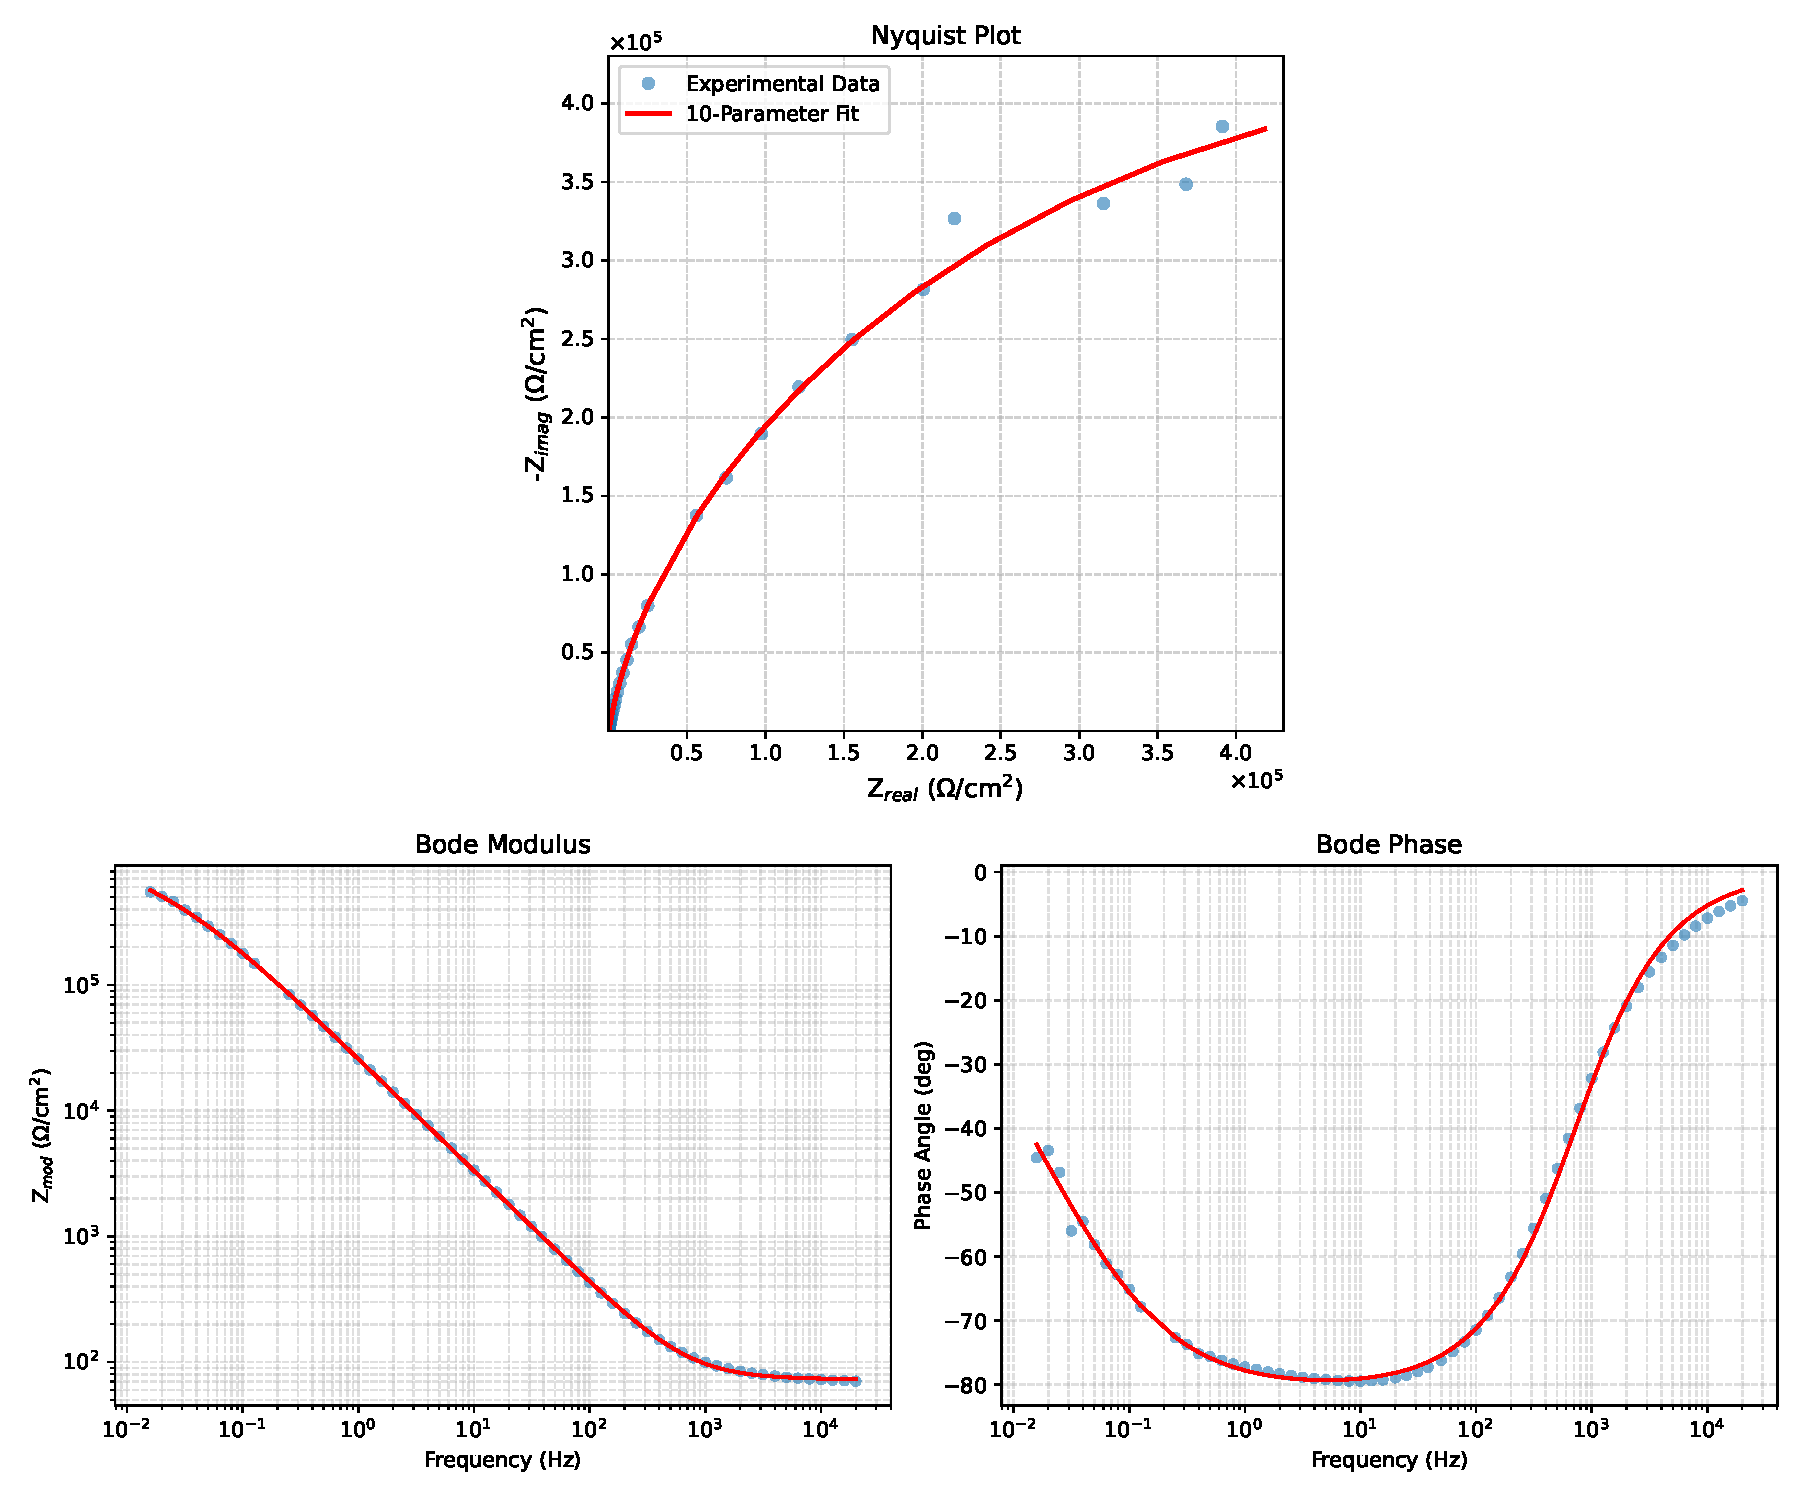
\includegraphics[width=0.7\textwidth]{plots_Cauvel_1_MBT_24H_2RC.pdf}
    \captionof{figure}{EIS Fit Results for Cauvel\_1\_MBT\_24H}
\end{center}

\newpage
\section*{Analysis Results: 48H}
\begin{center}
    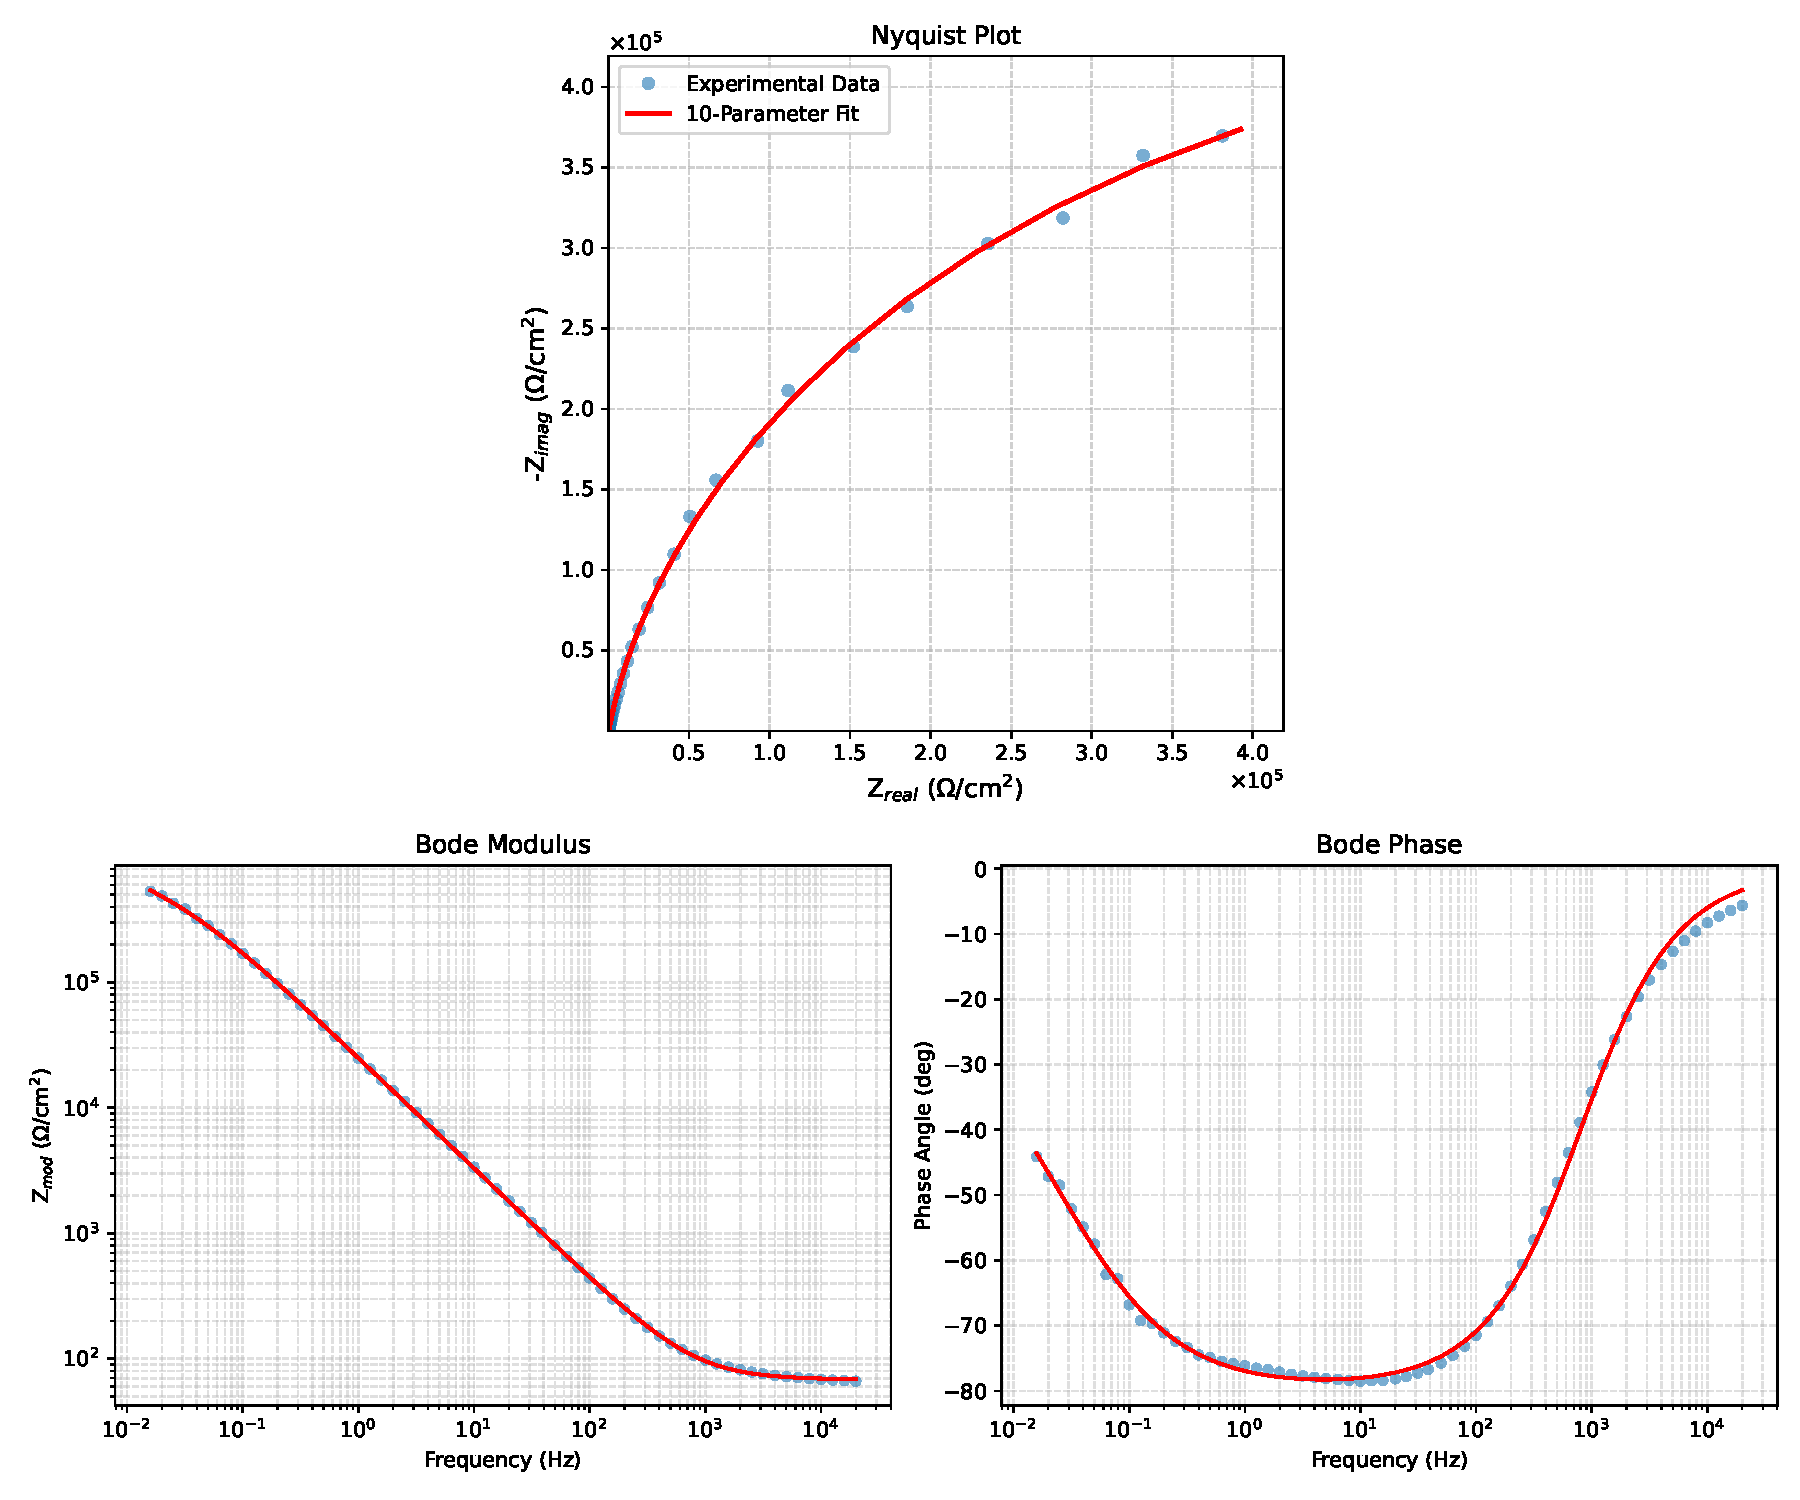
\includegraphics[width=0.7\textwidth]{plots_Cauvel_1_MBT_48H_2RC.pdf}
    \captionof{figure}{EIS Fit Results for Cauvel\_1\_MBT\_48H}
\end{center}

\newpage
\section*{Analysis Results: 72H}
\begin{center}
    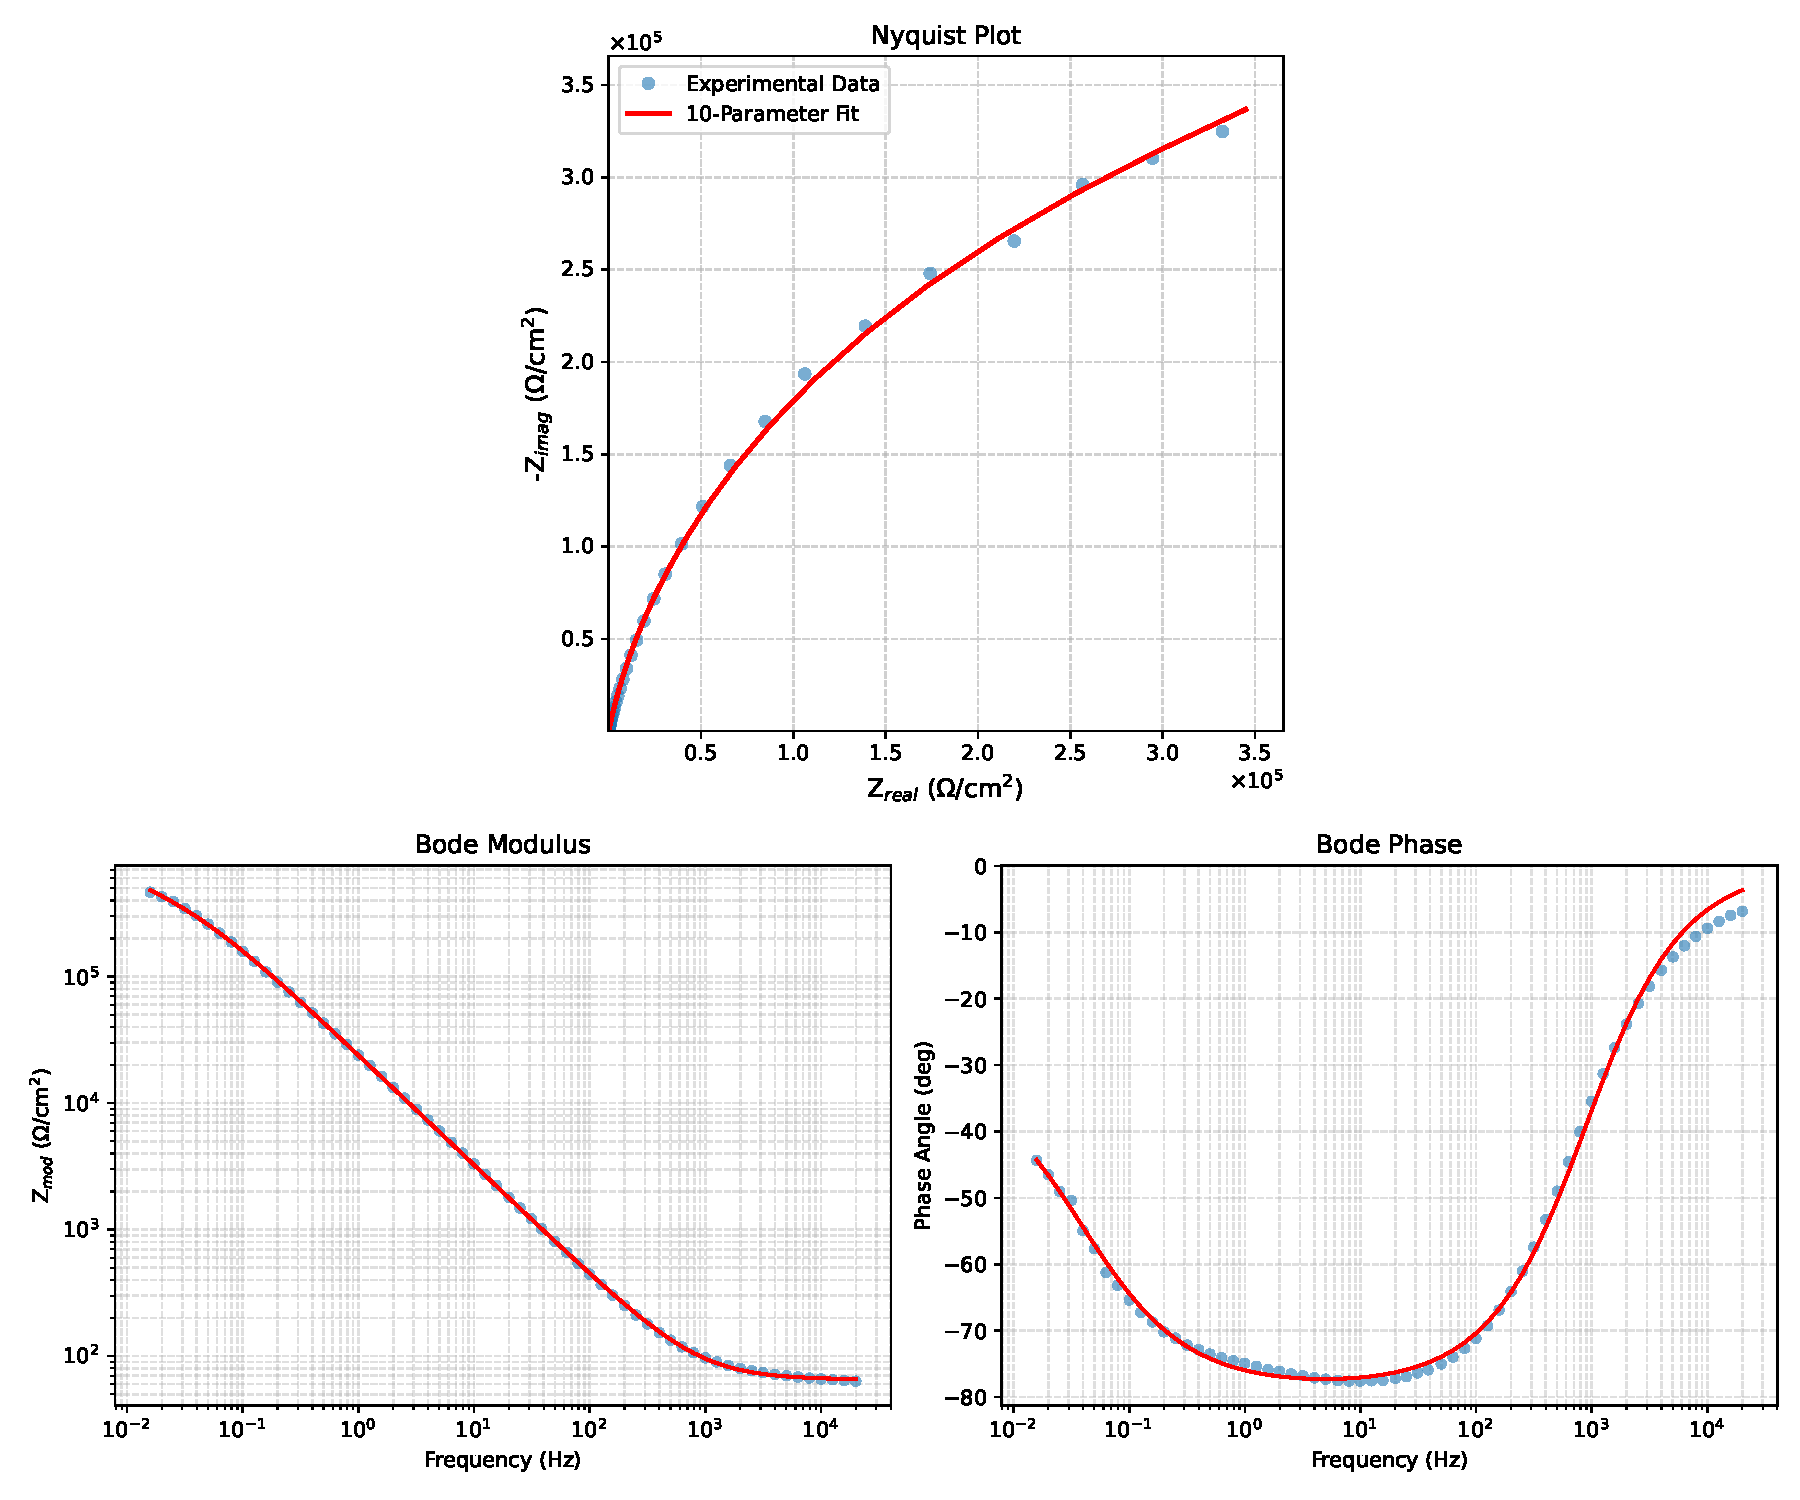
\includegraphics[width=0.7\textwidth]{plots_Cauvel_1_MBT_72H_2RC.pdf}
    \captionof{figure}{EIS Fit Results for Cauvel\_1\_MBT\_72H}
\end{center}

\newpage
\section*{Analysis Results: 168H}
\begin{center}
    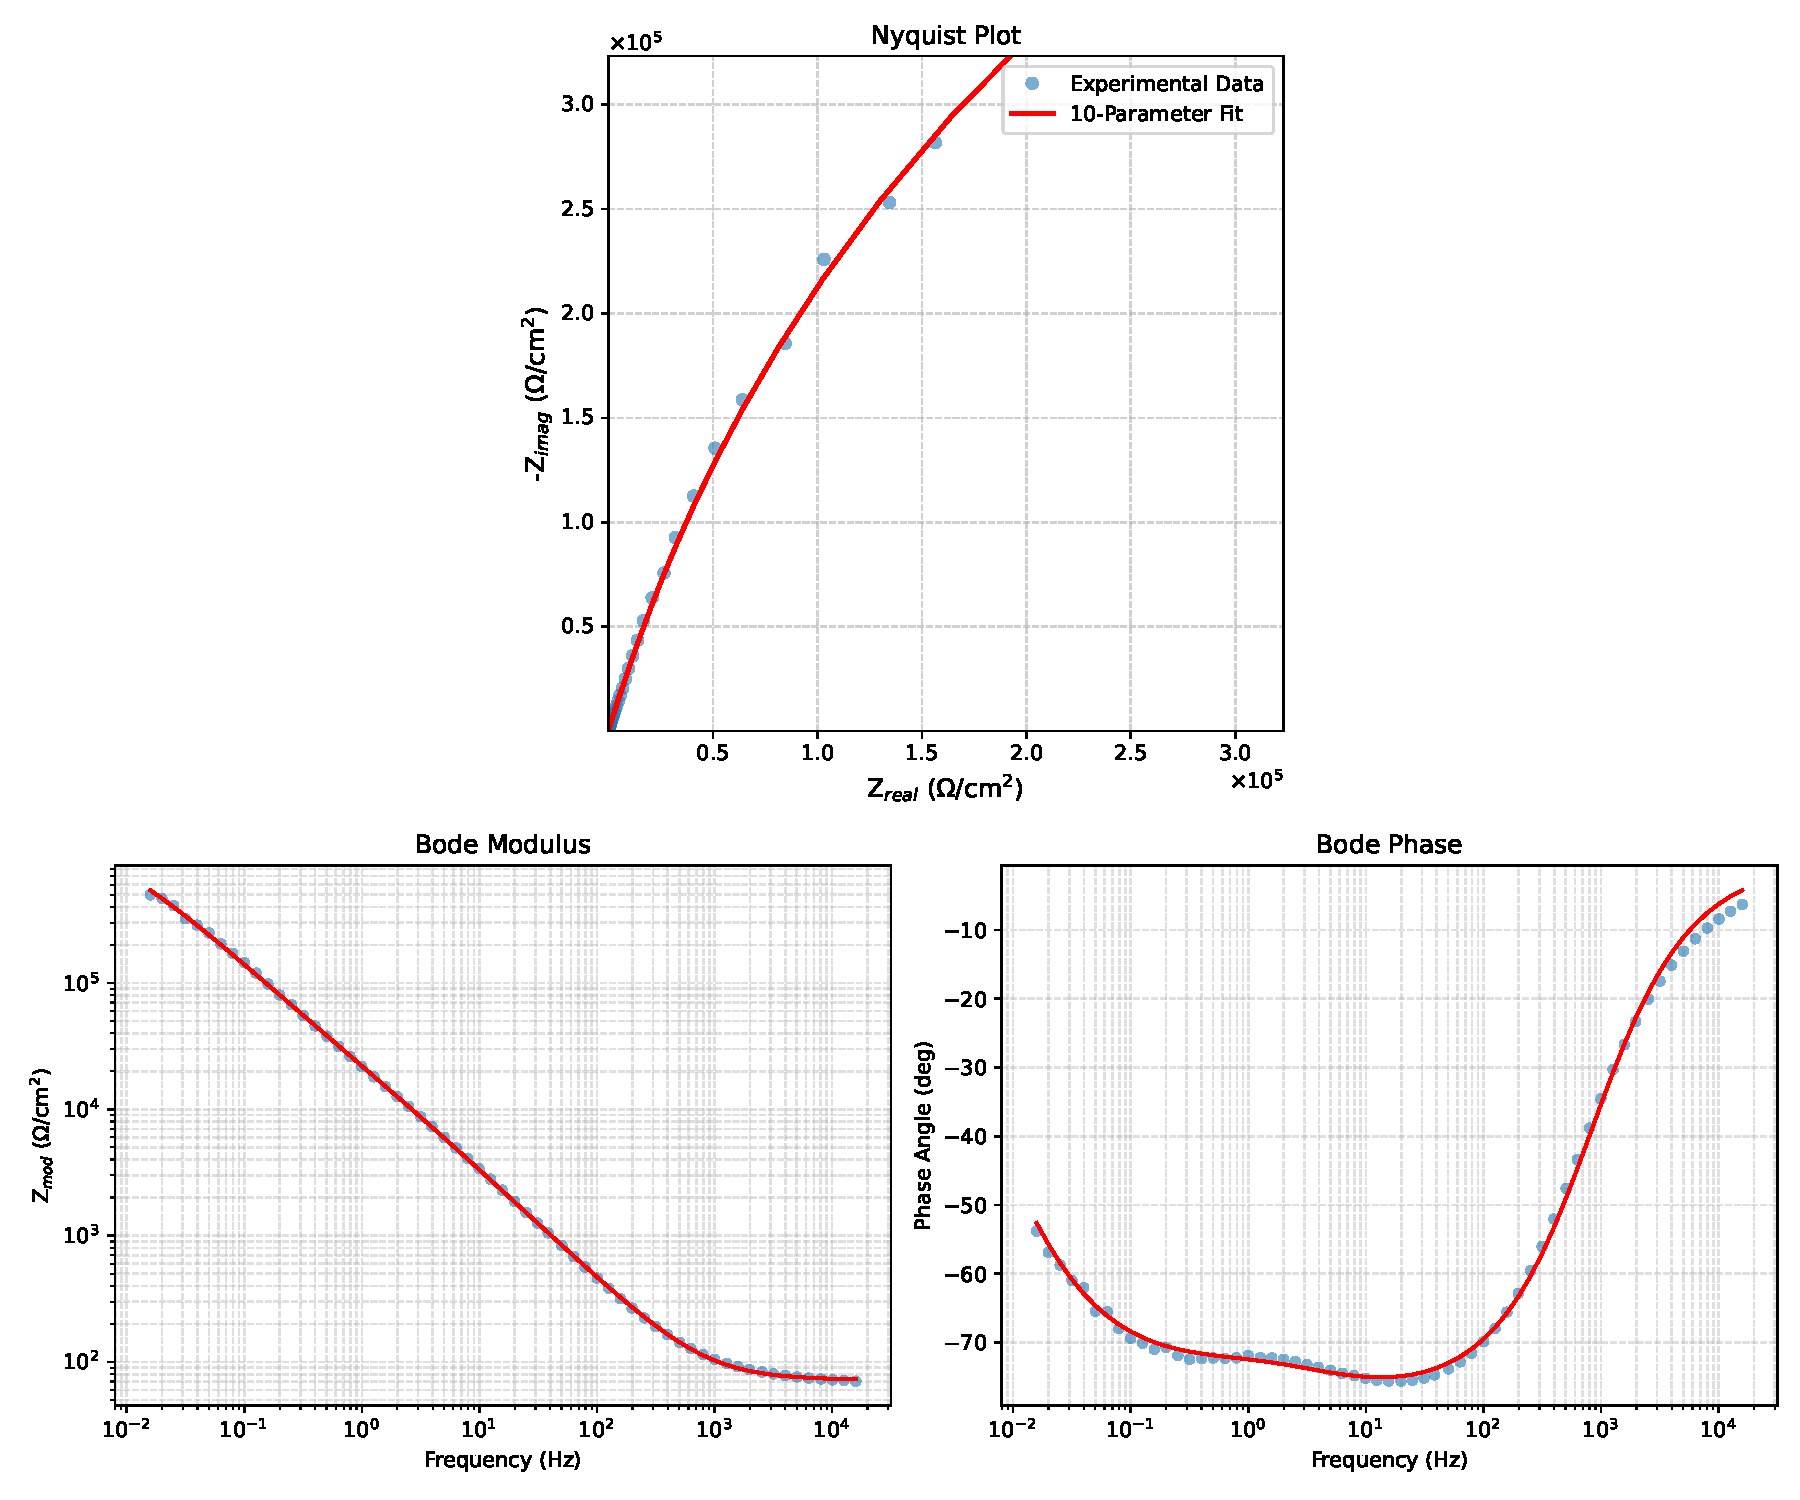
\includegraphics[width=0.7\textwidth]{plots_Cauvel_1_MBT_168H_2RC.pdf}
    \captionof{figure}{EIS Fit Results for Cauvel\_1\_MBT\_168H}
\end{center}


\end{document}
